\chapter{Implementacja metod akceleracji i~rezultaty pomiarów}
\label{sec:methods-results}

W rozdziale tym opisane zostały sposoby implementacji badanych metod akceleracji obliczeń oraz zaprezentowany zostały rezultaty przeprowadzonych testów wydajności. Wskazane zostały również wszelkie aspekty, na które trzeba zwrócić uwagę w~procesie budowania bibliotek z~daną metodę akceleracji oraz ich możliwości i~ograniczenia. Wszystkie wyniki pomiarów porównane zostały do wykonania sekwencyjnego w~C++, a~dla pozostałych metod akceleracji na wykresach kolorem szarym zaznaczony został zakres czasów wykonania sekwencyjnego wszystkich środowisk języka JavaScript.

Jak już wcześniej wspomniano w~rozdziale \ref{sec:benchmark}, dla każdej z~metod akceleracji zaimplementowano trzy algorytmy. Niżej przedstawiono nazwy i~oznaczenia używane na potrzeby implementacji i~prezentacji wyników.

\begin{itemize}
    \item Standard Hough Transform (SHT \textit{non-LUT}, \lstinline{SHT_Simple}) -- algorytm detekcji linii wykorzystujący intensywne obliczenia z~użyciem funkcji trygonometrycznych.
    \item Standard Hough Transform (SHT \textit{LUT}, \lstinline{SHT_Simple_Lookup}) -- algorytm detekcji linii wykorzystujący tablicę LUT do zapisanie potrzebnych wartości funkcji trygonometrycznych.
    \item Circle Hough Transform (CHT, \lstinline{CHT_Simple}) -- algorytm detekcji okręgów wykorzystujący metodę gradientu w~celu redukcji złożoności obliczeniowej (rozmiaru akumulatora). Zmienny parametr maksymalnego promienia obliczany jest ze wzoru $r_{max} = 20+10n$, gdzie $n$ to współczynnik inkrementowany w~kolejnych iteracjach pomiarów.
\end{itemize}


\section{Wykonanie sekwencyjne}

Implementacja procesu budowania biblioteki z~algorytmem transformacji w~wariancie wykonania sekwencyjnego nie wymagała zmian w~procesie budowania w~porównaniu do biblioteki \textit{benchmark}, będącej punktem odniesienia. Na rysunku \ref{plot:sequential} pokazano rezultaty pomiarów czasu wykonania w~postaci wykresów dla każdego z~implementowanych algorytmów.

\subsection{Wyniki pomiarów}

We wszystkich wariantach transformacji implementacja w~C++ osiągnęła najlepsze czasy wykonania, co jest oczekiwanym rezultatem. Dla algorytmu SHT najlepiej zoptymalizowanym okazało się środowisko przeglądarki Google Chrome będące \tms{3.71} wolniejsze od implementacji w~C++ dla wariantu \textit{non-LUT} i~$S_\theta = 1$. Dla wszystkich algorytmów środowiska serwerowe NodeJS oraz Deno osiągnęło porównywalne wyniki z~minimalną przewagą środowiska NodeJS, która była powtarzalna pomiędzy wieloma uruchomieniami testów, jednak jest pomijalnie mała. Najgorzej zoptymalizowana okazuje się przeglądarka Mozilla Firefox, będąc \tms{1.71} wolniejszą od Google Chrome dla $S_\theta = 1$. Interesującym dla niej zjawiskiem jest optymalizacja zachodząca dla SHT \textit{LUT} i~$S_\theta \geq 5$. 



\begin{figure}
    \groupBenchmark{
        \plotBenchmark{cpp_theta_SHT_Simple.csv}{cppColor}{{}}
        \addlegendentry{C++}

        \plotBenchmark{js-sequential_theta_SHT_Simple_node.csv}{nodeColor}{{}}
        \addlegendentry{Node}

        \plotBenchmark{js-sequential_theta_SHT_Simple_deno.csv}{denoColor}{{}}
        \addlegendentry{Deno}

        \plotBenchmark{js-sequential_theta_SHT_Simple_Firefox.csv}{firefoxColor}{{}}
        \addlegendentry{Firefox}

        \plotBenchmark{js-sequential_theta_SHT_Simple_Chrome.csv}{chromeColor}{{}}
        \addlegendentry{Chrome}

    } {
        \plotBenchmark{cpp_theta_SHT_Simple_Lookup.csv}{cppColor}{{}}
        \addlegendentry{C++}

        \plotBenchmark{js-sequential_theta_SHT_Simple_Lookup_node.csv}{nodeColor}{{}}
        \addlegendentry{Node}

        \plotBenchmark{js-sequential_theta_SHT_Simple_Lookup_deno.csv}{denoColor}{{}}
        \addlegendentry{Deno}

        \plotBenchmark{js-sequential_theta_SHT_Simple_Lookup_Firefox.csv}{firefoxColor}{{}}
        \addlegendentry{Firefox}

        \plotBenchmark{js-sequential_theta_SHT_Simple_Lookup_Chrome.csv}{chromeColor}{{}}
        \addlegendentry{Chrome}
    } {
        \plotBenchmark{cpp_theta_CHT_Simple.csv}{cppColor}{{}}
        \addlegendentry{C++}

        \plotBenchmark{js-sequential_theta_CHT_Simple_node.csv}{nodeColor}{{}}
        \addlegendentry{Node}

        \plotBenchmark{js-sequential_theta_CHT_Simple_deno.csv}{denoColor}{{}}
        \addlegendentry{Deno}

        \plotBenchmark{js-sequential_theta_CHT_Simple_Firefox.csv}{firefoxColor}{{}}
        \addlegendentry{Firefox}

        \plotBenchmark{js-sequential_theta_CHT_Simple_Chrome.csv}{chromeColor}{{}}
        \addlegendentry{Chrome}
    }
    [3400][850][14]
    \caption{Wyniki pomiarów czasu wydajności dla wykonania sekwencyjnego SHT i CHT.}
    \label{plot:sequential}
\end{figure}


Analizując różnice pomiędzy wykonaniami wariantów \textit{non-LUT} i~\textit{LUT} widać, że wszystkie środowiska zyskują na optymalizacji związanej z~używaniem zmiennych do przechowywania wartości funkcji trygonometrycznych, ponieważ optymalizacja ta stanowi jedyną różnicę w~implementacji. Jednak przeglądarka Mozilla Firefox zdecydowanie gorzej radzi sobie z~wykorzystaniem tej optymalizacji, co prowadzi do zwiększenia przewagi NodeJS i~Deno z~\tms{1.05} do \tms{1.99} większego czasu wykonania dla $S_\theta = 1$.

Dla algorytmu CHT środowiska NodeJS i~Deno, jak i~przeglądarka Google Chrome dają porównywalne rezultaty. Również i~tutaj przeglądarka Mozilla Firefox okazała się być wolniejsza od pozostałych środowisk wykonując ten sam algorytm na tych samych danych.

Na rysunku \ref{fig:profiler-seq} widać wynik profilowania wykonania sekwencyjnego algorytmu CHT dla $n=1$. Biblioteka \textit{benchmark} w~wewnętrznej metodzie \lstinline{waitForSteadyState} czeka, aż czas wykonania kodu się ustabilizuje. Pozwala to silnikowi JavaScript optymalizować czas wykonania, co w~pokazanych wynikach profilowania dzieje się w~blokach \textit{Optimize Code}, które występują tylko na początku pomiarów.

\begin{figure}[h]
    \centering
    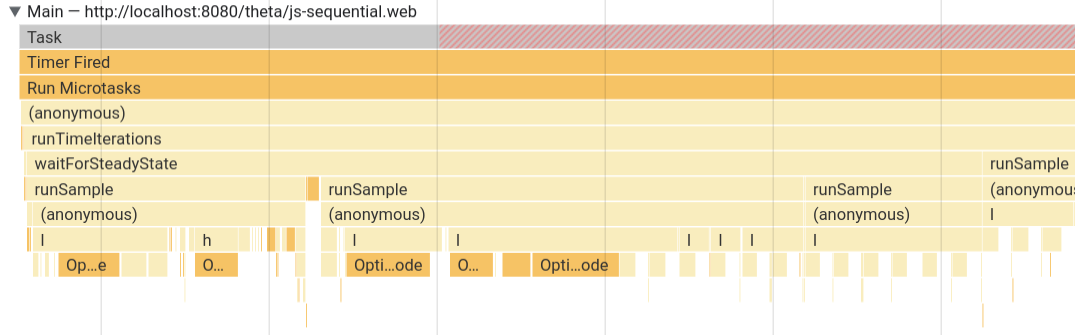
\includegraphics[width=\linewidth]{img/seq-profiler.png}
    \caption{Wynik profilowania wykonania sekwencyjnego algorytmu CHT w~przeglądarce Google Chrome.}
    \label{fig:profiler-seq}
\end{figure}

Zbadano również różnicę pomiędzy wartościami akumulatorów, która pomiędzy wariantami \textit{non-LUT} i~\textit{LUT} powinna być równa zero. Wykryto jednak różnicę dla jednego piksela, która widoczna jest na rysunku \ref{fig:diff:seq_lut}. Pochodzić ona może z~różnicy w~precyzji operacji zmiennoprzecinkowych. Tablica LUT funkcji trygonometrycznych zbudowana została z~wykorzystaniem pojedynczej precyzji i~obiektu tablicy typu \lstinline{Float32Array}. JavaScript wewnętrznie do reprezentacji liczb zmiennoprzecinkowych używa podwójnej precyzji.


\begin{figure}[h]
    \begin{subfigure}{0.3\textwidth}
        
\includegraphics[width=\linewidth] {../../packages/js-benchmarks/img/diff_seq_seq_lookup.png}
        \caption{SHT Sekwencyjny \textit{LUT}}\label{fig:diff:seq_lut}
    \end{subfigure}\hfill
    \begin{subfigure}{0.3\textwidth}
        
\includegraphics[width=\linewidth] {../../packages/js-benchmarks/img/diff_seq_wasm.png}
        \caption{SHT WASM}\label{fig:diff:wasm}
    \end{subfigure}\hfill
    \begin{subfigure}{0.3\textwidth}
        
\includegraphics[width=\linewidth] {../../packages/js-benchmarks/img/diff_seq_gpu.png}
        \caption{SHT WebGL}\label{fig:diff:gpu}
    \end{subfigure}
    \caption{Znormalizowana do przedziału $\lbrack 0, 255\rbrack$ absolutna różnica wartości akumulatorów z~wynikiem głosowania pomiędzy wykonaniem sekwencyjnym SHT \textit{non-LUT}.}\label{fig:diff}
\end{figure}



\section{NodeJS Native C++ Addon}

Implementacja natywnego modułu w~środowisku NodeJS wymaga utworzenia, oprócz właściwego kodu w~języku C++ oraz warstwy abstrakcji, która zapewnia obsługę interfejsu po stronie języka JavaScript, pozwala na określenie typów zmiennych, kopiowanie danych, czy wywoływanie funkcji. Warstwa ta zaimplementowana została za pomocą Node-API, która dostarcza niezbędne interfejsy i~funkcje w~języku C++, aby efektywnie powiązać kod C++ i~JavaScript~\cite{napi}. Implementacja natywnych modułów korzysta dokładnie z~tego samego kodu, dla którego przeprowadzony pomiary w~natywnym C++. Kod ten został skompilowany do postaci bibliotek współdzielonych, które w~procesie linkowania są dołączane do natywnego modułu NodeJS. 

Na listingu \ref{fig:nodejs} przedstawiony został plik z~paczki \textit{node-cpp-sequential}, który dołącza nagłówki z~paczki \textit{cpp-sequential}. Funkcja \lstinline{Napi::Object Init(Napi::Env env, Napi::Object exports)} zwraca obiekt, który definiuje wartości eksportowane przez moduł. W~niej właśnie definiowane są funkcje takie jak \lstinline{SHTSimple}, której implementację stanowi \lstinline{SHTSimpleBind}. Funkcja ta odpowiedzialna jest za stworzenie obiektów z~danymi wejściowymi zgodnie z~interfejsem dołączanych bibliotek (\lstinline{getTestImage} oraz \lstinline{getSHTOptions}), wywołania właściwej funkcji oraz zbudowanie obiektu z~odpowiedzią (\lstinline{getSHTResultBind}).

\begin{lstlisting}[language=C++, float=h, caption=Plik powiązania kodu C++ z~JavaScript, label=lst:cpp-js]
#define NAPI_DISABLE_CPP_EXCEPTIONS
#include "CHTSimple.h"
#include "SHTSimple.h"
#include "SHTSimpleLookup.h"
#include "napi.h"
#include <cstdint>

using namespace Napi;
    
Napi::Object SHTSimpleBind(const Napi::CallbackInfo &info) {
    Napi::Env env = info.Env();
    auto testImageBind = info[0].As<Napi::Uint8Array>();
    auto testImage = getTestImage(testImageBind);
    auto optionsBind = info[1].As<Napi::Object>();
    SHTOptions options = getSHTOptions(optionsBind);
    SHTResults results = SHTSimple(testImage, options);
  
    return getSHTResultBind(env, options, results);
  }
// ...
Napi::Object Init(Napi::Env env, Napi::Object exports) {
    exports.Set(Napi::String::New(env, "SHTSimple"),
                Napi::Function::New(env, SHTSimpleBind));
    // ...
    return exports;
}
  
NODE_API_MODULE(addon, Init)
\end{lstlisting}



\begin{figure}
    \groupBenchmark{
        \plotBenchmark{cpp-addon_theta_SHT_Simple_node.csv}{nodeColor}{{}}
        \addlegendentry{Node}

        \seqReference
    } {
        \plotBenchmark{cpp-addon_theta_SHT_Simple_Lookup_node.csv}{nodeColor}{{}}
        \addlegendentry{Node}

        \seqReferenceLookup
    }[1600][650]
    \label{plot:gpu}
    \caption{Node C++ addon SHT execution benchmark results.}
\end{figure}


\subsection{Wyniki pomiarów}

Na rysunku \ref{plot:cpu-addon} widać, że wykorzystanie tej metody akceleracji w~każdym przypadku przyspieszyło działania algorytmu względem odpowiadającego mu wykonania sekwencyjnego w~środowisku NodeJS. Przyspieszenie nastąpiło również względem wszystkich innych środowisk poza przypadkiem wariantu SHT \textit{LUT}, gdzie wydajność osiągnęła poziom wydajności odpowiednika wykonania sekwencyjnego w~przeglądarce Google Chrome.

Wariant SHT \textit{LUT} był \tms{4.40} szybszy od SHT \textit{non-LUT}, co wraz z~wynikami algorytmu CHT pozwala wyciągnąć wniosek, że jeśli w~algorytmie nie znamy z~góry niezbędnych wartości funkcji trygonometrycznych lub obliczenia są oparte głównie na liczbach całkowitych, to wykorzystanie tej metody akceleracji przynosi poprawę wydajności algorytmów. Oczywiście nie można zapominać o~wadach takiego rozwiązania, jaką stanowi konieczność implementacji warstwy wiążącej obydwa języki. Istnieje również konieczność zapewnienia kompatybilności biblioteki z~różnymi środowiskami uruchomieniowymi, dla których biblioteka musi zostać zbudowana zawczasu, lub w~momencie instalacji.

\section{WebAssembly i~asm.js}

Budowanie biblioteki wykorzystujące WebAssembly, tak jak w~przypadku natywnych modułów NodeJS, wymaga wykorzystania specyficznych narzędzi. Do budowy biblioteki we wszystkich wariantach wykorzystany został Emscripten \cite{emscripten} - zestaw narzędzi, dzięki którym dowolny przenośny kod w~językach kompatybilnych z~backendem kompilatora LLVM może został skompilowany do WebAssembly. Możliwym stało się uruchamianie w~środowiskach webowych kodu języków takich jak Python czy Lua, poprzez kompilację interpreterów tych języków.

\subsection{Implementacja procesu budowania}

Na listingu \ref{lst:wasm-build} przedstawiono wywołanie komendy \lstinline{emcc}, które inicjuje proces kompilacji. Z~perspektywy modularności oraz wygody użytkowania niezbędne jest omówienie opcji dostarczonych do komendy. Flaga \lstinline{--bind} uruchamia narzędzie Embind i~dodaje do kodu wynikowego modułu powiązania pomiędzy funkcjami eksportowanymi przez moduł, a~tymi zdefiniowanymi w~kodzie C++. Na listingu \ref{lst:wasm-bind} pokazano część kodu definiującego warstwę powiązania obydwu języków. Aby zapewnić zgodność z~docelowym interfejsem funkcja \lstinline{SHTSimpleBind} eksportowana jest jako \lstinline{SHTSimple}. W~porównaniu do natywnych modułów NodeJS w~tym wypadku Embind sam zajmuje się przetwarzaniem obiektów wejściowych na podstawie dostarczonych odwzorowań (linijka 16) i~powiązane funkcje zamiast argumentu z~całym kontekstem, otrzymać mogą argumenty w~docelowych typach. Jednak również tutaj wszystkie dane muszą zostać skopiowane do liniowego modelu pamięci WebAssembly. Za przetwarzanie obrazu wejściowego do postaci wektora liczb w~formacie \lstinline{uint8_t} odpowiedzialna jest funkcja \lstinline{emscripten::convertJSArrayToNumberVector}, która wymusza traktowanie wartości jako liczby, wpływając pozytywnie na wydajność. Opcja \lstinline{ALLOW_MEMORY_GROWTH=1} umożliwia powiększenie obszaru pamięci, który domyślnie ma rozmiar 16.0MB, co może nie wystarczyć, aby pomieścić przestrzeń akumulatora dla większych wartości próbkowania. Aby wynik kompilacji funkcjonował jako biblioteka eksportująca moduł ES6, należy użyć flag \lstinline{--no-entry} oraz opcji \lstinline{EXPORT_ES6=1}, \lstinline{MODULARIZE} oraz \lstinline{SINGLE_FILE=1}, aby binarny kod WebAssembly był zagnieżdżony w~pliku \lstinline{*.mjs} w~postaci kodu \textit{base64}. Nie można również zapomnieć o~możliwościach optymalizacji samego kompilatora, czyli o~flagach \lstinline{-O3}, czy \lstinline{-ffast-math}, która wprowadza optymalizacje działań matematycznych rezygnując z~poprawności wyników na ostatnich bitach.

\begin{lstlisting}[language=bash, float=ht, label=lst:wasm-build, caption=Komenda wykorzystana podczas kompilacji kodu C++ do modułu WebAssembly., showstringspaces=false]
COMMON_ARGS="-Inode_modules/cpp-sequential/include 
    --bind \
    -s MODULARIZE \
    -s ALLOW_MEMORY_GROWTH=1 \
    -s FILESYSTEM=0 \
    -s SINGLE_FILE=1 \
    -s ENVIRONMENT=web \
    -s EXPORT_ES6=1 \
    --no-entry \
    -std=c++17\
    -ffast-math\
    -O3"

### Non-SIMD
NON_SIMD_ARGS="$COMMON_ARGS \
    src/wasm_sequential.cc \
    node_modules/cpp-sequential/src/SHTSimpleLookup.cpp \
    node_modules/cpp-sequential/src/SHTSimple.cpp \
    node_modules/cpp-sequential/src/CHTSimple.cpp"

emcc $(echo $NON_SIMD_ARGS -o build/wasmSequential.mjs)
\end{lstlisting}

\begin{lstlisting}[language=C++, float=ht, label=lst:wasm-bind, caption=Wybrane fragmenty kodu warstwy powiązania WASM pomiędzy C++ i~JavaScript.]
// ...
#include <emscripten.h>
#include <emscripten/bind.h>

extern "C" {
// ...
EMSCRIPTEN_KEEPALIVE
SHTResults SHTSimpleBind(emscripten::val binaryImageBind, SHTOptions options) {
  auto testImage =
      emscripten::convertJSArrayToNumberVector<uint8_t>(binaryImageBind);
  return SHTSimple(testImage, options);
}
// ...
}

EMSCRIPTEN_BINDINGS(wasm_sequential) {
  emscripten::register_vector<uint32_t>("VectorUint32");
  emscripten::register_vector<uint8_t>("VectorUint8");
  emscripten::value_object<SHTSamplingOptions>("SHTSamplingOptions")
      .field("rho", &SHTSamplingOptions::rho)
      .field("theta", &SHTSamplingOptions::theta);
  // ...
  emscripten::function("SHTSimple", &SHTSimpleBind);
  // ...
}
\end{lstlisting}

\subsection{Warianty testów}

Dla każdego wariantu algorytmu transformacji przewidziano pomiary wydajności dla każdej z~wymienionych niżej metod.

\begin{itemize}
    \item asm.js -- wydajny podzbiór języka JavaScript zoptymalizowany pod kątem możliwości optymalizacji silnika i~inferencji typów,
    \item WASM -- standardowy wynik kompilacji kodu C++
    \item WASM SIMD (implicite) -- wynik kompilacji kodu C++ z~włączonym procesem automatycznej wektoryzacji wykonania, w~celu wykorzystania instrukcji wektorowych SIMD,
    \item WASM SIMD (explicite) -- wynik kompilacji kodu C++ z~ręcznie przeprowadzonym procesem wektoryzacji wykonania.
\end{itemize}

Zbudowanie biblioteki w~asm.js wymaga dodania opcji \lstinline{WASM=0}. Wariant SIMD explicite i~implicite budowany jest z~dodatkową flagą \lstinline{-msimd128}. Wariant SIMD explicite jest ręcznie przystosowany do obsługi operacji na wektorowych rejestrach 128b. Przykładem takiego zastosowania jest pokazana na listingu \ref{lst:simd} funkcja obliczająca minimalne i~maksymalne współrzędne w~przestrzeni akumulatora za jednym razem dla osi OX i~OY. W~procesie implementacji wersji SIMD explicite wykorzystano operacje na czteroelementowych wektorach liczb całkowitych bądź zmiennoprzecinkowych dla każdej intensywnie obliczeniowo pętli redukując liczbę ich iteracji czterokrotnie.

\begin{lstlisting}[language=C++, float=ht, label=lst:simd, caption=Funkcja \lstinline{getBounds} algorytmu CHT z~wykorzystaniem instrukcji SIMD.]
#include <wasm_simd128.h>
/ ...
void getBounds(int32_t x, int32_t max, v128_t vRBounds, int32_t *out) {
  v128_t vZero = wasm_i32x4_const_splat(0);
  v128_t vMax = wasm_i32x4_splat(max);
  v128_t vX = wasm_i32x4_splat(x);
  vX = wasm_i32x4_add(vRBounds, vX);
  vX = wasm_i32x4_max(vX, vZero);
  vX = wasm_i32x4_min(vX, vMax);
  wasm_v128_store(out, vX);
}
\end{lstlisting}

\subsection{Wyniki pomiarów}

Analizując wykres przedstawiający wyniki pomiarów czasów wykonania algorytmów z~wykorzystaniem kompilacji do asm.js przedstawiony na rysunku \ref{plot:asm} zobaczyć można, że ta metoda akceleracji w~każdym przypadku daje gorsze rezultaty od wykonania sekwencyjnego. Może to mieć dwie potencjalne przyczyny. Pierwszą z~nich jest nieprzeprowadzanie kompilacji kodu przez środowiska, które z~asm.js nie są w~pełni kompatybilne, co w~przypadku tych konkretnych algorytmów powoduje utratę wydajności. W~zbudowanym module nie znajdują się funkcje trygonometryczne \lstinline{Math.sin} i~\lstinline{Math.cos}. Oznacza to, że w~kodzie znajduje się ich ręczna implementacja, która nie korzysta z~biblioteki standardowej. Drugim możliwym powodem, w~szczególności w~przypadku przeglądarki Mozilla Firefox, która z~asm.js jest w~pełni kompatybilna, może być problem z~wykrywaniem kodu asm.js, który jest umieszczony w~jednej paczce z~resztą kodu w~procesie budowania. Świadczyć może o~tym fakt, że podczas profilowania wykonania nie występowały bloki \textit{Compile}, co ma miejsce podczas wykonania wyizolowanych przykładów.



\begin{figure}[ht]
    \groupBenchmark{
        \plotBenchmark{js-asm_theta_SHT_Simple_node.csv}{nodeColor}{{}}
        \addlegendentry{Node}

        \plotBenchmark{js-asm_theta_SHT_Simple_Firefox.csv}{firefoxColor}{{}}
        \addlegendentry{Firefox}

        \plotBenchmark{js-asm_theta_SHT_Simple_Chrome.csv}{chromeColor}{{}}
        \addlegendentry{Chrome}

        \seqReference
    } {
        \plotBenchmark{js-asm_theta_SHT_Simple_Lookup_node.csv}{nodeColor}{{}}
        \addlegendentry{Node}

        \plotBenchmark{js-asm_theta_SHT_Simple_Lookup_Firefox.csv}{firefoxColor}{{}}
        \addlegendentry{Firefox}

        \plotBenchmark{js-asm_theta_SHT_Simple_Lookup_Chrome.csv}{chromeColor}{{}}
        \addlegendentry{Chrome}

        \seqReferenceLookup
    }{
        \plotBenchmark{js-asm_theta_CHT_Simple_node.csv}{nodeColor}{{}}
        \addlegendentry{Node}

        \plotBenchmark{js-asm_theta_CHT_Simple_Firefox.csv}{firefoxColor}{{}}
        \addlegendentry{Firefox}

        \plotBenchmark{js-asm_theta_CHT_Simple_Chrome.csv}{chromeColor}{{}}
        \addlegendentry{Chrome}

        \seqReferenceCircle
    }[9000][2300][25]
    \caption{Wyniki pomiarów czasu wydajności dla wykonania SHT i CHT z wykorzystaniem kompilacji do asm.js.}
    \label{plot:asm}
\end{figure}


\begin{figure}[h]
    \groupBenchmark{
        \plotBenchmark{js-wasm_theta_SHT_Simple_node.csv}{nodeColor}{{}}
        \addlegendentry{Node}

        \plotBenchmark{js-wasm_theta_SHT_Simple_Firefox.csv}{firefoxColor}{{}}
        \addlegendentry{Firefox}

        \plotBenchmark{js-wasm_theta_SHT_Simple_Chrome.csv}{chromeColor}{{}}
        \addlegendentry{Chrome}

        \seqReference
    } {
        \plotBenchmark{js-wasm_theta_SHT_Simple_Lookup_node.csv}{nodeColor}{{}}
        \addlegendentry{Node}

        \plotBenchmark{js-wasm_theta_SHT_Simple_Lookup_Firefox.csv}{firefoxColor}{{}}
        \addlegendentry{Firefox}

        \plotBenchmark{js-wasm_theta_SHT_Simple_Lookup_Chrome.csv}{chromeColor}{{}}
        \addlegendentry{Chrome}

        \seqReferenceLookup
    } {
        \plotBenchmark{js-wasm_theta_CHT_Simple_node.csv}{nodeColor}{{}}
        \addlegendentry{Node}

        \plotBenchmark{js-wasm_theta_CHT_Simple_Firefox.csv}{firefoxColor}{{}}
        \addlegendentry{Firefox}

        \plotBenchmark{js-wasm_theta_CHT_Simple_Chrome.csv}{chromeColor}{{}}
        \addlegendentry{Chrome}

        \seqReferenceCircle
    }[2500][950][15]
    \caption{Wyniki pomiarów czasu wydajności dla wykonania SHT i CHT z wykorzystaniem kompilacji do WASM.}
    \label{plot:wasm}
\end{figure}


\begin{figure}[h]
    \groupBenchmark{
        \plotBenchmark{js-wasm_simd_explicit_theta_SHT_Simple_node.csv}{nodeColor}{{}}
        \addlegendentry{Node}

        \plotBenchmark{js-wasm_simd_explicit_theta_SHT_Simple_Firefox.csv}{firefoxColor}{{}}
        \addlegendentry{Firefox}

        \plotBenchmark{js-wasm_simd_explicit_theta_SHT_Simple_Chrome.csv}{chromeColor}{{}}
        \addlegendentry{Chrome}

        \seqReference
    } {
        \plotBenchmark{js-wasm_simd_explicit_theta_SHT_Simple_Lookup_node.csv}{nodeColor}{{}}
        \addlegendentry{Node}

        \plotBenchmark{js-wasm_simd_explicit_theta_SHT_Simple_Lookup_Firefox.csv}{firefoxColor}{{}}
        \addlegendentry{Firefox}

        \plotBenchmark{js-wasm_simd_explicit_theta_SHT_Simple_Lookup_Chrome.csv}{chromeColor}{{}}
        \addlegendentry{Chrome}

        \seqReferenceLookup
    }{
        \plotBenchmark{js-wasm_simd_explicit_theta_CHT_Simple_node.csv}{nodeColor}{{}}
        \addlegendentry{Node}

        \plotBenchmark{js-wasm_simd_explicit_theta_CHT_Simple_Firefox.csv}{firefoxColor}{{}}
        \addlegendentry{Firefox}

        \plotBenchmark{js-wasm_simd_explicit_theta_CHT_Simple_Chrome.csv}{chromeColor}{{}}
        \addlegendentry{Chrome}

        \seqReferenceCircle
    }[2200][650][15]
    \caption{Wyniki pomiarów czasu wydajności dla wykonania SHT i CHT z wykorzystaniem kompilacji do WASM z ręczną implementacją instrukcji SIMD.}
    \label{plot:wasm_simd_explicit}
\end{figure}


Kompilacja do WebAssembly zwiększyła wydajność wariantu algorytmu SHT \textit{non-LUT} we wszystkich testowanych środowiskach (rys. \ref{plot:wasm}). Jednak największy wpływ miała na środowiska przeglądarek internetowych, które zdają się lepiej reagować na te metodę akceleracji niż środowisko NodeJS. W~wariancie SHT \textit{LUT} za to nie zaobserwowano żadnej poprawy względem wykonania sekwencyjnego. dodatkowo nie zaobserwowano optymalizacji czasu wykonania dla $S_\theta \geq 5$. Warianty te różnią się jedynie zmniejszoną liczbą wywołać funkcji trygonometrycznych. Założyć można zatem, że zaobserwowana optymalizacja przeglądarki Mozilla Firefox dotyczyła właśnie ich i~nie odbyła w~momencie kompilacji do WebAssembly. 

Przypadek algorytmu CHT pokazuje jak różne środowiska mogą reagować na ten sam kod. W~przeglądarce Google Chrome z~silnikiem V8 zaobserwowano poprawę wydajności, gdzie wykonanie z~wykorzystaniem WebAssembly było \tms{1.70} szybsze od wykonania sekwencyjnego dla $n = 1$. Mozilla Firefox jednak zachowuje się inaczej. Dla $n = 1$ wykonanie z~wykorzystaniem WebAssembly było \tms{1.63} szybsze, niż wykonanie sekwencyjne, jednak dla $n = 10$ czas wykonania był już taki sam jak czas wykonania sekwencyjnego. Na tej podstawie można wyciągnąć wniosek, że w~przypadku przeglądarki Mozilla Firefox duża liczba iteracji generuje narzut, który niweluje korzyści, jakie płyną z~ogólnej poprawny wydajności dzięki WebAssembly. 

Kompilacja do WebAssembly z~włączonym procesem automatycznej wektoryzacji w~narzędziu Emscripten nie przyniosła żadnej różnicy w~porównaniu do wykonania zwykłego kodu WebAssembly i~dlatego nie będzie dalej omawiana. Natomiast w~przypadku ręcznej optymalizacji, czego przykład pokazany został na listingu \ref{lst:simd}, poprawa wydajności zależała od środowiska. Na rysunku \ref{plot:wasm_simd_explicit} zaobserwować można, że wszystkie środowiska pozytywnie zareagowały na zastosowaną metodę dla wariantu algorytmu SHT \textit{non-LUT}. Najszybsza znów okazała się przeglądarka Google Chrome, osiągając wynik \tms{1.50} lepszy od wykonania sekwencyjnego. W~wariancie SHT \textit{LUT} jednak wykonanie sekwencyjne było \tms{1.15} szybsze. Wykonanie wariantu CHT w~przeglądarka Mozilla Firefox, w~porównaniu do wykonania sekwencyjnego, było wolniejsza, a~wykonanie w~środowiskach Google Chrome i~NodeJS zyskało na wydajności.

Dla analizowanego kąta obrotu $\theta = \frac{\pi}{2}$ wykryto duże różnice w~akumulatorze pomiędzy wykonaniem SHT WASM a~sekwencyjnym SHT. Różnica widoczna jest na rysunku \ref{fig:diff:wasm}. Oprócz wyraźnej linii różnica występuje też dla wielu pojedynczych pól akumulatora i~może wynikać z~różnicy w~reprezentacji w~algorytmie liczb zmiennoprzecinkowych, co generuje różnice w~wyliczeniach pól akumulatora.

\section{Współbieżność}

Zrównoleglenie wykonania bezdyskusyjnie przynosi wzrost wydajności. Jednak, aby mogło być zastosowane algorytm musi dać się zrównoleglić. Również docelowe środowiska muszą tę współbieżność wspierać. Wspólnym mianownikiem wszystkich badanych środowisk jest wielowątkowość w~postaci Worker'ów. Oprócz nich środowisko NodeJS posiada natywne mechanizmy komunikacji między procesami, jednak nie są one przedmiotem badań tej pracy.

Komunikacja pomiędzy Worker'ami odbywa się z~wykorzystaniem interfejsów WebWorker API. Dostarczają one mechanizm wiadomości, które są asynchronicznie przetwarzane przez Worker'y, które jako niezależne wątki mają osobną pętlę zdarzeń. Wiadomość jest w~abstrakcji przetwarzania zdarzeniem. Metoda \lstinline{Worker.postMessage(...)} oraz definiowana funkcja \lstinline{self.onmessage} pozwala na wysyłanie i~obsługę zdarzeń wiadomości pomiędzy wątkami. Mechanizm ten jest bardzo prosty, niweluje problemy wyścigów oraz współdzielenia zasobów, ponieważ wszystkie dane są albo kopiowane, albo transferowane z~jednego wątku do drugiego. Jego wadą jest sam interfejs, który wymaga tworzenia dodatkowych mechanizmów serializacji i~parsowania złożonych wiadomości. Z~pomocą przychodzi, zastosowana przy implementacji Worker'ów na potrzeby badan, biblioteka Comlink \cite{comlink}. Pozwala ona na zdalne wywoływanie funkcji i~synchronizację zmiennych, co nie odbiega interfejsem od sposobu interakcji z~metodami i~atrybutami standardowych obiektów. Jest ona kompatybilna ze wszystkimi badanymi środowiskami. 

Implementacja Worker'ów wymagała przystosowania algorytmów. Podzielono wykonanie głównych ich pętli pomiędzy wątki. W~testach badano czasy wykonania dla liczby wątków $c=4$. Aby zapewnić kompatybilność ze wszystkimi środowiskami konieczne było zbudowanie dwóch wersji biblioteki. Biblioteka w~środowisku Deno była uruchamiana z~pominięciem procesu budowania, ponieważ Deno pozwala bezpośrednio na uruchomienie kodu w~języku TypeScript. 

Dla środowiska przeglądarki internetowej konieczne jest użycie loader'a \lstinline{worker-loader}, który, z~opcją \lstinline{inline: 'no-fallback'}, odpowiedzialny jest za dołączenie kodu Worker'a do kodu biblioteki, aby taka biblioteka mogła być ponownie zbudowana razem z~docelową aplikacją. W~standardowym scenariuszu, kiedy Worker budowany jest razem z~aplikacją, jego kod jest pobierany jako osobny plik przez przeglądarkę. Kod musi być dołączony w~tym samym pliku, ponieważ niemożliwym jest, bez dodatkowych skryptów, wskazanie i~skopiowanie pliku Worker'a w~procesie budowania.

Dla środowiska NodeJS konieczne jest jawne wskazanie środowiska, dla którego przeznaczona jest budowana biblioteka poprzez ustawienie opcji \lstinline{target: 'node'}. NodeJS do obsługi Worker'ów używa wbudowanego modułu, WebWorker API jest lekko zmodyfikowane, a~konstruktor obiektu \lstinline{Worker} nie jest dostępny jako symbol globalny. Narzędzie Webpack musi uwzględnić wszystkie te elementy. Niekompatybilność ta uniemożliwia w~wypadku tej metody akceleracji zbudowanie pliku kompatybilnego ze wszystkimi środowiskami. Na rysunku \ref{fig:workers-struct} przedstawiono diagram zależności modułów w~kodzie, w~tym adapterów, które zapewniają kompatybilność kodu algorytmu ze wszystkimi środowiskami. Kod części właściwego algorytmu, który tworzy i~wywołuje funkcje Worker'ów w~środowisku Deno jest oderwany od jego odpowiednika wspólnego dla przeglądarek i~NodeJS. Jest to spowodowane niekompatybilnością API biblioteki Comlink w~wersji na środowisko Deno.

\begin{figure}[h]
    \centering
    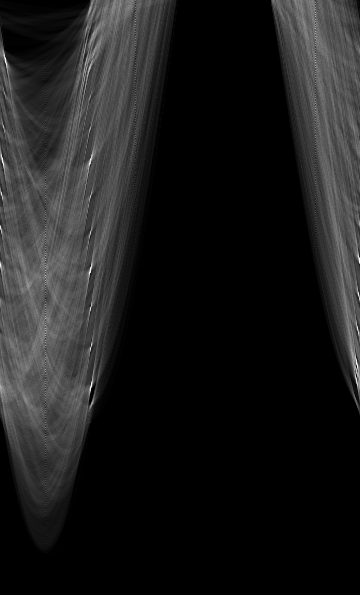
\includegraphics[width=\linewidth]{diagrams/out/workers.png}
    \caption{Sieć zależności pomiędzy modułami implementującymi algorytm SHT w~wersji \textit{non-LUT}, która zapewnia kompatybilność ze wszystkimi środowiskami.}
    \label{fig:workers-struct}
\end{figure}

\subsection{Wyniki pomiarów}

Pomiary dla wykonania wielowątkowego przeprowadzone były przy przeznaczonych do tego 4 fizycznych rdzeniach procesora, aby uniknąć wpływu hyper-threading'u na czas wykonania. Wymagało to przypisania 8 wirtualnych rdzeni używając maski \lstinline{0x000000ff} jako konfiguracji narzędzia \lstinline{taskset}.



\begin{figure}
    \groupBenchmark{
        \plotBenchmark{js-workers_theta_SHT_Simple_node.csv}{nodeColor}{{}}
        \addlegendentry{Node}

        \plotBenchmark{js-workers_theta_SHT_Simple_deno.csv}{denoColor}{{}}
        \addlegendentry{Deno}

        \plotBenchmark{js-workers_theta_SHT_Simple_Firefox.csv}{firefoxColor}{{}}
        \addlegendentry{Firefox}

        \plotBenchmark{js-workers_theta_SHT_Simple_Chrome.csv}{chromeColor}{{}}
        \addlegendentry{Chrome}

        \seqReference
    } {
        \plotBenchmark{js-workers_theta_SHT_Simple_Lookup_node.csv}{nodeColor}{{}}
        \addlegendentry{Node}

        \plotBenchmark{js-workers_theta_SHT_Simple_Lookup_deno.csv}{denoColor}{{}}
        \addlegendentry{Deno}

        \plotBenchmark{js-workers_theta_SHT_Simple_Lookup_Firefox.csv}{firefoxColor}{{}}
        \addlegendentry{Firefox}

        \plotBenchmark{js-workers_theta_SHT_Simple_Lookup_Chrome.csv}{chromeColor}{{}}
        \addlegendentry{Chrome}

        \seqReferenceLookup
    }[1700][500]
    \label{plot:workers}
    \caption{Workers SHT execution benchmark results with concurrency $n=4$. Gray area shows sequential JavaScript execution performance range. Non-LUT variant performs better than sequential execution. On the other hand the LUT one has gained only small increase in performance.}
    % TODO: speedup math
\end{figure}


\begin{wraptable}{r}{6cm}
    \caption{Speedup metrics for worker acceleration method ($S_\theta = 1, p = 4$).}
    \label{tab:worker_speedup}
    \setlength{\tabcolsep}{0.5em}
    \begin{tabular}{lrr}%
        \hline
        Env.        & Speedup & Efficiency              \\
        \hline
        Chrome      & 2.99    & 0.75                    \\
        Firefox     & 2.82    & 0.70                    \\
        Node        & 3.25    & \textcolor{green!70!black}{0.81} \\
        Deno        & 2.70    & \textcolor{red}{0.67}   \\
        Chrome \textit{LUT}  & 1.85    & 0.46                    \\
        Firefox \textit{LUT} & 1.89    & 0.47                    \\
        Node \textit{LUT}    & 1.76    & 0.44                    \\
        Deno \textit{LUT}    & 1.51    & \textcolor{red}{0.38}   \\
        \hline
    \end{tabular}
\end{wraptable}

Na rysunku \ref{plot:workers} pokazane zostały wykresy z~wynikami pomiarów czasów wykonania z~wykorzystaniem czterech Worker'ów. Jak w~większości przypadków również i~tutaj, dla obydwu wariantów SHT, prym we wzroście wydajności wiedzie przeglądarka Google Chrome. Przy krótszych czasach wykonania dla wariantu CHT uwydatnia się większa niż dla poprzednich metod wartość odchylenia standardowego. Szczególnie widoczna jest w~przypadku przeglądarki Mozilla Firefox. Spowodowane jest to asynchronicznością komunikacji z~Worker'em, gdzie wiadomości nie są obsługiwane od razu, a~trafiają do pętli zdarzeń. W~zależności od implementacji, jak i~liczby zdarzeń do obsłużenia przez pętlę, czasy te mogą się różnić. Kod Worker'ów jest również osobno optymalizowany, co zwiększa skalę zjawiska zimnego startu w~przypadku tej metody akceleracji.  Na rysunku \ref{fig:profiler-workers} widać wynik profilowania pierwszych wykonań kodu na stworzonych instancjach Worker'ów. W~pierwszych wykonaniach widać bloki \textit{Optimize Code}, a~dalsze wykonania wykonują się już po optymalizacji. Podczas długiej przerwy pomiędzy wykonaniami proces optymalizacji zachodził dla wątku głównego.

\begin{figure}[h]
    \centering
    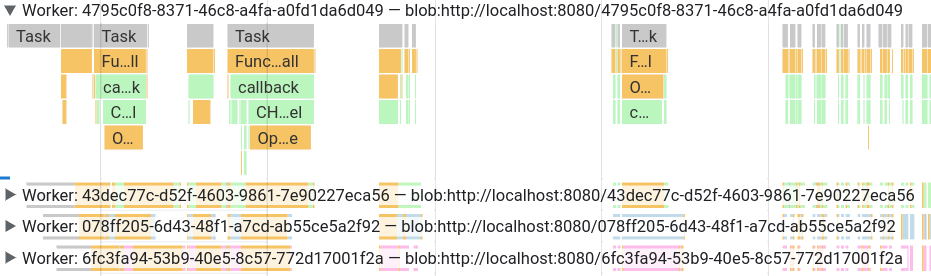
\includegraphics[width=\linewidth]{img/workers-profiler.png}
    \caption{Wynik profilowania wykonania algorytmu CHT w~przeglądarce Google Chrome z~użyciem Worker'ów.}
    \label{fig:profiler-workers}
\end{figure}

W tabeli \ref{tab:speedup} przedstawiono miarę przyspieszenia obliczeń oraz jej efektywność. Największe przyspieszenie, a~zarazem jego efektywność ma miejsce w~przypadku wariantu SHT \textit{non-LUT} i~środowiska NodeJS. Różnica wyników pomiędzy wariantami SHT \textit{non-LUT} i~SHT \textit{LUT} jest znacząca i~kolejny raz wskazuje na funkcje trygonometryczne i~liczby zmiennoprzecinkowe jako czynnik, na który trzeba zwrócić uwagę podczas optymalizacji algorytmów. W~wariancie CHT przyspieszenie jest niewielkie, ponieważ zrównolegleniu poddany został sam proces głosowania na środek okręgu. Jeśli w~danych wejściowych większa liczba pikseli byłaby zapalona, etap głosowania byłby bardziej wymagający, co zwiększyłoby efektywność przyspieszenia.

Worker'y współdzielą pamięć akumulatora w~postaci obiektu \lstinline{SharedArrayBuffer}. Z~uwagi na to, że każdy Worker działał na własnym fragmencie pamięci podczas procesu głosowania, nie było konieczne stosowanie operacji atomowych z~wykorzystaniem metod interfejsu \lstinline{Atomic}. Użycie takiego interfejsu spowalniało wykonanie algorytmu w~testach podczas implementacji. 


\section{GPGPU}

Implementacja akceleracji z~użyciem układu graficznego wymaga dostosowania algorytmu do masowego zrównoleglenia wydzielając funkcję jądra (kernel), która wykonywać się będzie równolegle na setkach rdzeni jednocześnie zawsze rozwijając wszystkie gałęzie wyrażeń warunkowych. Stworzona implementacja korzysta z~mechanizmów generowania grafiki WebGL API, co nakłada dodatkowe ograniczenia w~przeciwieństwie do standardowego podejścia. Kernel nie ma możliwości modyfikacji danych w~pamięci współdzielonej, a~jego jedynym wynikiem jest wektor liczb. W~zależności od algorytmu liczby te mogą być różnie interpretowane - jako zmienne logiczne, liczby stało i~zmiennoprzecinkowe, czy też w~standardowy sposób, jako kolor piksela.

\subsection{Standard Hough Transform}

Przystosowanie procesu głosowania dla wariantu SHT wymaga podejścia skoncentrowanego na generowaniu jednej wartości elementu akumulatora. Proces ten jest masowo zrównoleglony przez układ graficzny równolegle generując wszystkie wartości w~akumulatorze. 

Jeśli jeden piksel na obrazie odwzorowywany jest na sinusoidę w~przestrzeni akumulatora, a~jeden punkt w~przestrzeni akumulatora to jedna linia na obrazie, to odwrotnym podejściem do głosowania jest zliczenie, dla jednego elementu akumulatora, ile pikseli na obrazie przechodzi przez potencjalną linię, na którą może być on odwzorowany. Żeby uwzględnić wszystkie piksele linii, których zbocze $m > 1$, iteracja po przestrzeni obrazu odbywa się również w~wariancie, w~którym układ współrzędnych jest obrócony o~$90^\circ$. Dlatego równania (\ref{eq:gpuD}) i~(\ref{eq:gpuE}) obliczające sumę zapalonych pikseli zamieniają współrzędne $x$ i~$y$ miejscami w~zależności kąta nachylenia.
Końcowy wzór na wartość pola akumulatora przedstawiony został na równaniu (\ref{eq:gpuF}).
\begin{align}
    \rho(\theta) &= x\cos{\theta} + y\sin{\theta} \label{eq:gpuA} \\
    y_a(\rho,\theta,x) &= \frac{\rho-x\sin{\theta}}{\cos{\theta}} \label{eq:gpuB}\\
    x_a(\rho,\theta,y) &= \frac{\rho-y\cos{\theta}}{\sin{\theta}} \label{eq:gpuC}\\
    A_x(\rho, \theta) &= 
    \begin{cases} 
    \sum^{w-1}_{x=0}I(x, y_a(\rho,\theta,x)),&\rho \in \left[\frac{\pi}{4}, \frac{3\pi}{4}\right) \lor \rho \in \left[\frac{5\pi}{4}, \frac{7\pi}{4}\right) \\
    0,& \text{dla pozostałych }\rho
    \end{cases} \label{eq:gpuD}\\
    A_y(\rho, \theta) &= 
    \begin{cases} 
    \sum^{h-1}_{y=0} I(x_a(\rho,\theta,y), y),& \rho \in \left[0, \frac{\pi}{4}\right) \lor \rho \in \left[\frac{3\pi}{4}, \frac{5\pi}{4}\right) \lor \rho \in \left[\frac{7\pi}{4}, 2\pi\right) \\
    0,& \text{dla pozostałych }\rho
    \end{cases} \label{eq:gpuE}\\
    A(\rho, \theta) &= A_x(\rho, \theta) + A_y(\rho, \theta) \label{eq:gpuF}
\end{align}
\begin{eqexpl}
    \item{$x, y$} współrzędne piksela obrazu;
    \item{$I(x, y)$} wartość piksela obrazu.
    \item{$A_x, A_y$} częściowa zawartość akumulatora w~zależności od nachylenia zbocza prostej;
    \item{$A$} zawartość akumulatora.
    \item{$w, h$} szerokość i~wysokość obrazu;
    \item{$x_a, y_a$} funkcje obliczające drugą współrzędną linii na podstawie odwzorowania z~akumulatora;
    \item{$\rho$} odległość prostej od środka układu współrzędnych;
    \item{$\theta$} obrót prostej od wokół układu współrzędnych;
\end{eqexpl}
\vspace{0.5cm}


Zbudowanie biblioteki nie wymagało dodatkowych zmian konfiguracji bazowej narzędzia Webpack. Do implementacji obliczeń z~wykorzystaniem WebGL wykorzystano bibliotekę \textit{gpu.js}. Listing \ref{lst:gpu-sht} przedstawia funkcję tworzącą kernel dla wariantu SHT\textit{non-LUT}. Jedynym argumentem funkcji kernela jest tablica z~wejściowym obrazem. Pozostałe parametry dostarczane są jako stałe, co przyspiesza do nich dostęp. Sprawia to jednak, że dla każdego zestawu opcji istnieje konieczność stworzenia nowego kernela. W~implementowanym algorytmie kernele zapisywane są w~mapie, której kluczem są wartości opcji. Kernel zwraca jedną liczbę stanowiącą wynik równania (\ref{eq:gpuF}).

Na listingu również zobaczyć możemy utworzenie funkcji za pomocą konstruktora, która zwraca właściwa funkcję i~jest od razu wykonywana - \lstinline{new Function(`return function (testImage/* : number[] */){/*...*/}`)()}. Jest to niezbędne, aby mieć pełną kontrolę nad wejściem do mechanizmów transpilacji biblioteki \textit{gpu.js}, ponieważ kod w~procesie budowania biblioteki jest minifikowany, co zmienia nazwy zmiennych i~stosuje skrócone notacje, z~którymi biblioteka \textit{gpu.js} ma problem z~transpilacją. Na listingu \ref{lst:gpu-mini} widać przykład zminifikowanego kodu błędnie transpilowanego do języka ESSL, gdzie problem stanowi połączenie post-inkrementacji z~wyrażeniem logicznym.

\begin{lstlisting}[language=JavaScript, float=ht, label=lst:gpu-mini, caption=Przykład minifikacji kodu błędnie transpilowanego do języka ESSL przez bibliotekę \textit{gpu.js}.]
// before
if(offset < this.constants.width * this.constants.height &&
                testImage[offset] == 1) {
    acc+=1;
}
// after
t<this.constants.width*this.constants.height&&1==e[t]&&a++;
\end{lstlisting}

\begin{lstlisting}[language=JavaScript, float=ht, label=lst:gpu-sht, caption=Funkcja tworząca kernel dla wariantu SHT \textit{non-LUT}]

import { GPU, IKernelRunShortcutBase } from "gpu.js";

export const gpu = new GPU();
export function createSHTSimpleKernel(
    hsWidth: number, hsHeight: number, width: number, height: number,
    samplingRho: number, samplingTheta: number
) {
  return gpu
    .createKernel(
      new Function(`return function (testImage/* : number[] */) {
        // ...
        let acc = 0;
        // ...
        return acc;
      }`)(),
      {
        output: [hsWidth * hsHeight],
        constants: {hsWidth, width, height, samplingRho, samplingTheta},
      }
    )
    .setLoopMaxIterations(Math.max(width, height))
    .setOptimizeFloatMemory(true) as IKernelRunShortcutBase<Float32Array>;
}
\end{lstlisting}

\subsection{Circle Hough Transform}
\label{sec:cht-gpu}

W wariancie CHT zaimplementowano łącznie 3 kernele. Dwa z~nich odpowiedzialne są za obliczenie splotu obrazu z~operatorem Sobela, aby wyznaczyć gradient krawędzi. Pętle iterujące po macierzy 3x3 operatora zostały rozwinięte do sześciu wyrażeń w~celu redukcji narzutu związanego z~obsługą pętli. Kernele te zwracają wynik w~postaci obiektu tekstury, której powiązane dane znajdują się bezpośrednio na GPU. Tekstury te są następnie wejściem do kernela wyznaczającego wartość pola akumulatora w~procesie głosowania na środki okręgów. Dzięki takiemu złożeniu kerneli dane splotów nie przechodzą przez CPU, aby trafić z~powrotem do układ graficznego. Wartość piksela wyznaczana jest na podstawie liczby linii, o~długości wyznaczanej na podstawie maksymalnego i~minimalnego wyszukiwanego promienia, przechodzących przez dany punkt w~przestrzeni akumulatora.

\subsection{Wyniki pomiarów}

Na rysunku \ref{plot:gpu} przedstawiono wyniki pomiarów czasu wykonania algorytmów zaimplementowanych z~wykorzystaniem biblioteki \textit{gpu.js}. Widać, że metoda ta cechuje się bardzo niestabilnym z~odchyleniami od liniowego, czasem wykonania. Brak dużego odchylenia standardowego sugeruje, że czas zależeć może od ogólnego obciążenia systemu oraz od optymalizacji wykorzystanych zasobów procesora graficznego, co sugeruje podobny czas wykonania dla $S_\theta \in \{5,6,7\}$ w~wariancie SHT \textit{LUT}. Dla SHT w~każdym środowisku i~wariancie algorytmu udało się przyspieszyć czas wykonania bądź osiągnąć porównywalny względem wykonania sekwencyjnego w~języku C++. Przyspieszenie wynosi \tms{3.81} dla wariantu SHT \textit{non-LUT} i~oscyluje w~okolicy \tms{1} dla SHT \textit{LUT} oraz $S_\theta = 1$. Ze względu na odwrotne podejście do generowania wartości w~akumulatorze oraz na zmniejszoną precyzje obliczeń dla liczb zmiennoprzecinkowych w~procesorach graficznych, różnica pomiędzy wygenerowanym akumulatorem dla tej metody, a~wariantem sekwencyjnym jest znacząca i~została pokazana na rysunku \ref{fig:diff:gpu}. Nie wpływa ona jednak znacząco na ocenioną empirycznie jakość detekcji. 



\begin{figure}
    \groupBenchmark{
        %\plotBenchmark{js-gpu_theta_SHT_Simple_node.csv}{nodeColor}{{}}
        %\addlegendentry{Node}

        %\plotBenchmark{js-gpu_theta_SHT_Simple_deno.csv}{denoColor}{{}}
        %\addlegendentry{Deno}

        \plotBenchmark{js-gpu_theta_SHT_Simple_Firefox.csv}{firefoxColor}{{}}
        \addlegendentry{Firefox 95}

        \plotBenchmark{js-gpu_theta_SHT_Simple_Chrome.csv}{chromeColor}{{}}
        \addlegendentry{Chrome 97}

        \seqReference
    } {
        %\plotBenchmark{js-gpu_theta_SHT_Simple_Lookup_node.csv}{nodeColor}{{}}
        %\addlegendentry{Node}

        %\plotBenchmark{js-gpu_theta_SHT_Simple_Lookup_deno.csv}{denoColor}{{}}
        %\addlegendentry{Deno}

        \plotBenchmark{js-gpu_theta_SHT_Simple_Lookup_Firefox.csv}{firefoxColor}{{}}
        \addlegendentry{Firefox 95}

        \plotBenchmark{js-gpu_theta_SHT_Simple_Lookup_Chrome.csv}{chromeColor}{{}}
        \addlegendentry{Chrome 97}

        \seqReferenceLookup
    }[550][200]
    \label{plot:gpu}
    \caption{WebGL SHT execution benchmark results. Gray area shows sequential JavaScript execution performance range.}
\end{figure}


Wąskim gardłem w~metodach akceleracji z~wykorzystaniem układów graficznych jest komunikacja CPU z~GPU. Wysyłanie i~odbieranie danych zajmuje nieproporcjonalnie dużo czasu, co widać na rysunku \ref{fig:profiler-gpu}. Widać na nim również proces transpilacji kodu kernela (bloki \lstinline{createKernel} i~\lstinline{build}). Konieczność zbudowania kernela zwiększa czas zimnego startu, który jest szczególnie duży w~przypadku tej metody akceleracji, co zostanie opisane w~sekcji \ref{sec:coldstart}.


\begin{figure}[h]
    \centering
    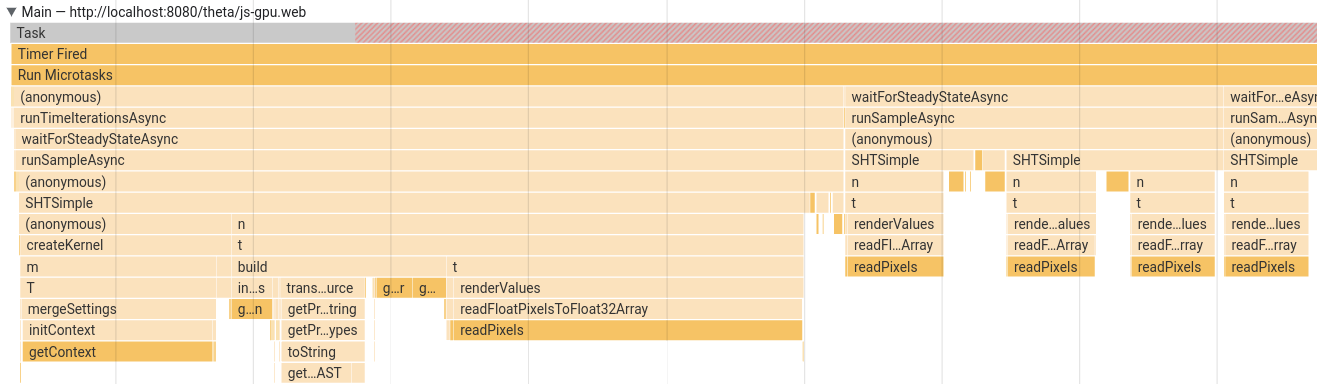
\includegraphics[width=\linewidth]{img/gpu-profiler.png}
    \caption{Wynik profilowania wykonania algorytmu CHT w~przeglądarce Google Chrome z~wykorzystaniem biblioteki \textit{gpu.js}.}
    \label{fig:profiler-gpu}
\end{figure}


W przypadku wersji CHT nie udało się uzyskać przyspieszenia, a~dodatkowo implementacja w~taki sam sposób zwiększyła złożoność obliczeniową, która stała się ponad-liniowa. Dla każdego punktu akumulatora wszystkie punkty wokół niego na obrazie, nie dalej niż maksymalnie szykany promień, muszą zostać sprawdzone pod kątem generowania linii, która przecina generowany punkt akumulatora. Na tej podstawie można oszacować złożoność jako $O(n^2)$. Dla dużych promieni rzędu 220 pikseli, czas wykonania potrafi wynieść 25s. W~ramach pracy nie analizowano dalej tego problemu, a~wszelkie próby poprawy złożoności algorytmu nie przyniosły efektu. Doświadczenia z~udaną akceleracją wariantu SHT algorytmu pozwala sądzić, że zaimplementowanie wersji z~jednym trójwymiarowym akumulatorem przyniosłoby oczekiwane rezultaty. Ograniczeniem w~takiej implementacji byłby rozmiar akumulatora. W~obydwu przeglądarkach maksymalny rozmiar wyjścia to $16384\times16384$. Rozwiązaniem tego problemu może być podział wykonania na części, gdzie każda z~nich generuje maksymalny możliwy fragment akumulatora.

\section{Problem zimnego startu}
\label{sec:coldstart}

Problem zimnego startu związany jest z~narzutem czasowym występującym przy uruchomieniu środowiska, kompilacji i~optymalizacji kodu, czy też uruchomienia dodatkowych mechanizmów obsługujących wątki lub komunikację z~GPU. W~zależności od sytuacji może być on pomijalny, ale i~krytyczny. Pominąć można go w~procesie prototypowania, kiedy wielokrotnie uruchamiamy środowisko po zamianach w~algorytmie co jakiś czas. Wtedy dodatkowy czas nie stanowi problemu, oczywiście jeśli jest akceptowalnie krótki. Krytyczny okazać się może w~produkcyjnych rozwiązaniach \textit{serverless}, gdzie każdemu wykonaniu funkcji towarzyszy osobna instancja środowiska, a~optymalizacje nie są przeprowadzane. Oczywiście w~zależności od obciążenia pojedyncza instancja środowiska może obsługiwać wiele zapytań, co przy odpowiednio długim czasie trwania pozwala na optymalizację kodu i~kompilację JIT.

Każda z~badanych metod akceleracji posiada inną charakterystykę zimnego startu. Na rysunku \ref{plot:coldstart-sht} i~\ref{plot:coldstart-sht-lut} przedstawiono czasy wykonania algorytmu SHT kolejno \textit{non-LUT} i~\textit{LUT} znormalizowane do przedziału $\left[0, 1\right]$ dla $S_\theta=1$. Pomiary wykonywano, dopóki współczynnik wariancji dla okna o~długości 5 był mniejszy lub równy 0.01. Na wykresach pokazano tylko sześć pierwszych pomiarów, ponieważ to dla nich występuje największa zmiana czasu wykonania. Widać, że największa różnica w~czasie występuje dla metod wywoływanych asynchronicznie - Worker'ów oraz WebGL. Metody te mają problem z~osiągnięciem stabilnych czasów również po stabilizacji wykrytej przez metrykę współczynnika wariancji.

Metody wykorzystujące WebAssembly nie zyskują na wydajności w~kolejnych pomiarach. Jest to zrozumiałe, ponieważ skompilowany kod nie jest już optymalizowany przez silnik. Oznacza to jednak również, że widocznej optymalizacji nie ulegają mechanizmy powiązania kodu JavaScript i~WebAssembly - głównie mechanizmy kopiowania danych. Dla wariantu SHT \textit{LUT}, dla metod akceleracji wykonujących kod JavaScript, wydać wyraźną poprawę wydajności w~kolejnych pomiarach. Kolejny raz widać zatem, że funkcje trygonometryczne i~ich wielokrotne wywoływanie spowalniają czas wykonania, a~dodatkowo wpływają negatywnie na optymalizację związaną z~pierwszymi uruchomieniami algorytmu w~ramach tej samej instancji środowiska.

\begin{figure}[h]
    \groupColdstart{
        \plotColdstart{coldstart/js-sequential_coldstart_SHT_Simple_Chrome.csv}{}
        \addlegendentry{JS Seq.}
        \plotColdstart{coldstart/js-asm_coldstart_SHT_Simple_Chrome.csv}{{}}
        \addlegendentry{asm.js}
        \plotColdstart{coldstart/js-wasm_coldstart_SHT_Simple_Chrome.csv}{{}}
        \addlegendentry{WASM}
        \plotColdstart{coldstart/js-wasm_simd_explicit_coldstart_SHT_Simple_Chrome.csv}{{}}
        \addlegendentry{WASM SIMD (expl.)}
        \plotColdstart{coldstart/js-workers_coldstart_SHT_Simple_Chrome.csv}{{}}
        \addlegendentry{Workers}
        \pgfplotsset{cycle list shift=1}
        \plotColdstart{coldstart/js-gpu_coldstart_SHT_Simple_Chrome.csv}{{}}
        \addlegendentry{WebGL}
    } {
        \plotColdstart{coldstart/js-sequential_coldstart_SHT_Simple_Firefox.csv}{}
        \addlegendentry{JS Seq.}
        \plotColdstart{coldstart/js-asm_coldstart_SHT_Simple_Firefox.csv}{{}}
        \addlegendentry{asm.js}
        \plotColdstart{coldstart/js-wasm_coldstart_SHT_Simple_Firefox.csv}{{}}
        \addlegendentry{WASM}
        \plotColdstart{coldstart/js-wasm_simd_explicit_coldstart_SHT_Simple_Firefox.csv}{{}}
        \addlegendentry{WASM SIMD (expl.)}
        \plotColdstart{coldstart/js-workers_coldstart_SHT_Simple_Firefox.csv}{{}}
        \addlegendentry{Workers}
        \pgfplotsset{cycle list shift=1}
        \plotColdstart{coldstart/js-gpu_coldstart_SHT_Simple_Firefox.csv}{{}}
        \addlegendentry{WebGL}
    } {
        \plotColdstart{coldstart/js-sequential_coldstart_SHT_Simple_node.csv}{}
        \addlegendentry{JS Seq.}
        \plotColdstart{coldstart/js-asm_coldstart_SHT_Simple_node.csv}{{}}
        \addlegendentry{asm.js}
        \plotColdstart{coldstart/js-wasm_coldstart_SHT_Simple_node.csv}{{}}
        \addlegendentry{WASM}
        \plotColdstart{coldstart/js-wasm_simd_explicit_coldstart_SHT_Simple_node.csv}{{}}
        \addlegendentry{WASM SIMD (expl.)}
        \plotColdstart{coldstart/js-workers_coldstart_SHT_Simple_node.csv}{{}}
        \addlegendentry{Workers}
    } {
        \plotColdstart{coldstart/js-sequential_coldstart_SHT_Simple_deno.csv}{}
        \addlegendentry{JS Seq.}
        \pgfplotsset{cycle list shift=3}
        \plotColdstart{coldstart/js-workers_coldstart_SHT_Simple_deno.csv}{{}}
        \addlegendentry{Workers}
    }
\caption{Wyniki pomiarów pierwszych czasów wykonania algorytmu SHT \textit{non-LUT} znormalizowane do przedziału $\left[0, 1\right]$ dla $S_\theta=1$.}
\label{plot:coldstart-sht}
\end{figure}

\begin{figure}[h]
    \groupColdstart{
        \plotColdstart{coldstart/js-sequential_coldstart_SHT_Simple_Lookup_Chrome.csv}{}
        \addlegendentry{JS Seq.}
        \plotColdstart{coldstart/js-asm_coldstart_SHT_Simple_Lookup_Chrome.csv}{{}}
        \addlegendentry{asm.js}
        \plotColdstart{coldstart/js-wasm_coldstart_SHT_Simple_Lookup_Chrome.csv}{{}}
        \addlegendentry{WASM}
        \plotColdstart{coldstart/js-wasm_simd_explicit_coldstart_SHT_Simple_Lookup_Chrome.csv}{{}}
        \addlegendentry{WASM SIMD (expl.)}
        \plotColdstart{coldstart/js-workers_coldstart_SHT_Simple_Lookup_Chrome.csv}{{}}
        \addlegendentry{Workers}
        \pgfplotsset{cycle list shift=1}
        \plotColdstart{coldstart/js-gpu_coldstart_SHT_Simple_Lookup_Chrome.csv}{{}}
        \addlegendentry{WebGL}
    } {
        \plotColdstart{coldstart/js-sequential_coldstart_SHT_Simple_Lookup_Firefox.csv}{}
        \addlegendentry{JS Seq.}
        \plotColdstart{coldstart/js-asm_coldstart_SHT_Simple_Lookup_Firefox.csv}{{}}
        \addlegendentry{asm.js}
        \plotColdstart{coldstart/js-wasm_coldstart_SHT_Simple_Lookup_Firefox.csv}{{}}
        \addlegendentry{WASM}
        \plotColdstart{coldstart/js-wasm_simd_explicit_coldstart_SHT_Simple_Lookup_Firefox.csv}{{}}
        \addlegendentry{WASM SIMD (expl.)}
        \plotColdstart{coldstart/js-workers_coldstart_SHT_Simple_Lookup_Firefox.csv}{{}}
        \addlegendentry{Workers}
        \pgfplotsset{cycle list shift=1}
        \plotColdstart{coldstart/js-gpu_coldstart_SHT_Simple_Lookup_Firefox.csv}{{}}
        \addlegendentry{WebGL}
    } {
        \plotColdstart{coldstart/js-sequential_coldstart_SHT_Simple_Lookup_node.csv}{}
        \addlegendentry{JS Seq.}
        \plotColdstart{coldstart/js-asm_coldstart_SHT_Simple_Lookup_node.csv}{{}}
        \addlegendentry{asm.js}
        \plotColdstart{coldstart/js-wasm_coldstart_SHT_Simple_Lookup_node.csv}{{}}
        \addlegendentry{WASM}
        \plotColdstart{coldstart/js-wasm_simd_explicit_coldstart_SHT_Simple_Lookup_node.csv}{{}}
        \addlegendentry{WASM SIMD (expl.)}
        \plotColdstart{coldstart/js-workers_coldstart_SHT_Simple_Lookup_node.csv}{{}}
        \addlegendentry{Workers}
    } {
        \plotColdstart{coldstart/js-sequential_coldstart_SHT_Simple_Lookup_deno.csv}{}
        \addlegendentry{JS Seq.}
        \pgfplotsset{cycle list shift=3}
        \plotColdstart{coldstart/js-workers_coldstart_SHT_Simple_Lookup_deno.csv}{{}}
        \addlegendentry{Workers}
    }
\caption{Wyniki pomiarów pierwszych czasów wykonania algorytmu SHT \textit{LUT} znormalizowane do przedziału $\left[0, 1\right]$ dla $S_\theta=1$.}
\label{plot:coldstart-sht-lut}
\end{figure}

\begin{figure}[h]
    \groupColdstart{
        \plotColdstart{coldstart/js-sequential_coldstart_CHT_Simple_Chrome.csv}{}
        \addlegendentry{JS Seq.}
        \plotColdstart{coldstart/js-asm_coldstart_CHT_Simple_Chrome.csv}{{}}
        \addlegendentry{asm.js}
        \plotColdstart{coldstart/js-wasm_coldstart_CHT_Simple_Chrome.csv}{{}}
        \addlegendentry{WASM}
        \plotColdstart{coldstart/js-wasm_simd_explicit_coldstart_CHT_Simple_Chrome.csv}{{}}
        \addlegendentry{WASM SIMD (expl.)}
        \plotColdstart{coldstart/js-workers_coldstart_CHT_Simple_Chrome.csv}{{}}
        \addlegendentry{Workers}
        \pgfplotsset{cycle list shift=1}
        \plotColdstart{coldstart/js-gpu_coldstart_CHT_Simple_Chrome.csv}{{}}
        \addlegendentry{WebGL}
    } {
        \plotColdstart{coldstart/js-sequential_coldstart_CHT_Simple_Firefox.csv}{}
        \addlegendentry{JS Seq.}
        \plotColdstart{coldstart/js-asm_coldstart_CHT_Simple_Firefox.csv}{{}}
        \addlegendentry{asm.js}
        \plotColdstart{coldstart/js-wasm_coldstart_CHT_Simple_Firefox.csv}{{}}
        \addlegendentry{WASM}
        \plotColdstart{coldstart/js-wasm_simd_explicit_coldstart_CHT_Simple_Firefox.csv}{{}}
        \addlegendentry{WASM SIMD (expl.)}
        \plotColdstart{coldstart/js-workers_coldstart_CHT_Simple_Firefox.csv}{{}}
        \addlegendentry{Workers}
        \pgfplotsset{cycle list shift=1}
        \plotColdstart{coldstart/js-gpu_coldstart_CHT_Simple_Firefox.csv}{{}}
        \addlegendentry{WebGL}
    } {
        \plotColdstart{coldstart/js-sequential_coldstart_CHT_Simple_node.csv}{}
        \addlegendentry{JS Seq.}
        \plotColdstart{coldstart/js-asm_coldstart_CHT_Simple_node.csv}{{}}
        \addlegendentry{asm.js}
        \plotColdstart{coldstart/js-wasm_coldstart_CHT_Simple_node.csv}{{}}
        \addlegendentry{WASM}
        \plotColdstart{coldstart/js-wasm_simd_explicit_coldstart_CHT_Simple_node.csv}{{}}
        \addlegendentry{WASM SIMD (expl.)}
        \plotColdstart{coldstart/js-workers_coldstart_CHT_Simple_node.csv}{{}}
        \addlegendentry{Workers}
    } {
        \plotColdstart{coldstart/js-sequential_coldstart_CHT_Simple_deno.csv}{}
        \addlegendentry{JS Seq.}
        \pgfplotsset{cycle list shift=3}
        \plotColdstart{coldstart/js-workers_coldstart_CHT_Simple_deno.csv}{{}}
        \addlegendentry{Workers}
    }
\caption{Wyniki pomiarów pierwszych czasów wykonania algorytmu CHT znormalizowane do przedziału $\left[0, 1\right]$ dla $n=1$.}
\label{plot:coldstart-cht}
\end{figure}


Analizując przyspieszenie związane z~optymalizacją na rysunku \ref{plot:coldstart-cht} przedstawiającym pierwsze czasy wykonania algorytmu CHT dla $n=1$, możemy zobaczyć dużo większe przyspieszenie dla kolejnych uruchomień niż dla algorytmów SHT. Z~racji na mniejszy rozmiar problemu i~krótszy czas iteracji implementacja ta lepiej pokazuje możliwości optymalizacji środowisk, ponieważ obliczenia nie są skupione tak bardzo na powtarzających się iteracjach. W~wariancie sekwencyjnym wspólną cechą środowisk opartych na silniku V8 jest zwiększenie czasu wykonania dla drugiego wywołania funkcji, gdzie kolejne są już optymalizowane. Widać dla metod wykorzystujących WebAssembly, optymalizację instrukcji wywołania modułów WebAssembly, która raz wykonana daje stałe czasy w~kolejnych wykonaniach algorytmu. Środowiska oparte na silniku V8 cechują się ogólną skutecznością w~optymalizacji kodu JavaScript w~porównaniu do silnika SpiderMonkey środowiska przeglądarki Mozilla Firefox.

\section{Przykład przetwarzania obrazu z~kamery w~przeglądarce internetowej}

Implementacja przetwarzania obrazu z~kamery w~przeglądarce wykonana została w~celu zbadania i~wykrycia ewentualnych problemów z~integracją zbudowanych bibliotek z~aplikacją SPA oraz z~procesem pozyskiwania obrazu z~kamery. Obraz na potrzeby testów dostarczany był w~formie strumieniowania plików \lstinline{*.mp4} o~rozdzielczości 720p do wirtualnego urządzenia kamery stworzonego w~wykorzystaniem narzędzia \textit{v4l2loopback}.

Pobranie obrazu z~kamery wymaga skorzystania z~WebRTC API, które pozwala uzyskać dostęp do kamery i~mikrofonu użytkownika i~zarządzać nimi w~abstrakcjach strumieni, które zawierają ścieżki audio i~wideo. Jednym ze standardowych sposobów na uzyskanie obrazu do przetworzenia jest utworzenie obiektu HTML5 \lstinline{<video/>} z~atrybutem \lstinline{srcObject}, który przyjąć musi wartość obiektu zwróconego przez zapytanie \lstinline{navigator.MediaDevices.getUserMedia(...)}. Następnie, na podstawie obiektu \lstinline{<video/>}, na obiekcie \lstinline{<canvas/>} narysować możemy wyświetlaną obecnie klatkę. Aby pobrać taką klatkę do przetwarzania w~formie binarnej pliku obrazu w~wybranym formacie należy użyć metody \lstinline{canvas.toBlob(...)}. Aby pobrać wartości konkretnych pikseli należy użyć metody kontekstu rysowania obiektu \lstinline{<canvas/>} - \lstinline{ctx.getImageData(...)}. 

Przechodząc od obrazu źródłowego z~kamery do wartości konkretnych pikseli musimy przejść przez formy pośrednie obiektu \lstinline{<video/>} i~\lstinline{<canvas/>}. Wpływa to na wydajność i~wygodę użytkowania, która jest zdecydowanie mniejsza, jeśli do niezbędnych operacji trzeba wykorzystać obiekty modelu DOM. Rozwiązaniem, które nie wykorzystuje modelu DOM jest zaimplementowane w~ramach przykładu ImageCapture API. Działa on jako wrapper ścieżki wideo pochodzącej z~strumienia uzyskanego za pomocą metody \lstinline{getUserMedia} i~dzięki metodzie \lstinline{grabFrame} możemy pobrać obiekt \lstinline{ImageBitmap}. Rozwiązanie to wciąż wykorzystuje obiekt \lstinline{<canvas/>} do narysowania na nim obrazu z~obiektu \lstinline{ImageBitmap}, a~następnie pobrania poszczególnych pikseli. ImageCapture API jest specyfikacją eksperymentalną, która wspierana jest tylko w~przeglądarkach opartych na Chromium.

Przetwarzanie zostało zaimplementowane dla obydwu algorytmów i~przetestowane z~dwoma obrazami wejściowymi (rys. \ref{fig:road-money}). Wejściem algorytmu detekcji kształtów wykorzystujący transformację Hough'a jest binarny obraz z~wykrytymi krawędziami. Obraz z~kamery musi zatem zostać pozyskany, narysowany na obiekcie \lstinline{<canvas/>}, przekształcony do skali szarości, a~następnie poddany operacji wykrywania krawędzi. Implementacja wykorzystuje bibliotekę \textit{image-js}\cite{image-js} oraz \textit{canny-edge-detector}\cite{canny}, które odpowiadają kolejno za ogólne przetwarzanie obrazów oraz za implementację operatora Canny, który służy do wykrywania krawędzi na obrazie. 

\begin{figure}
    \centering
    \begin{subfigure}{0.48\textwidth}
        \centering
        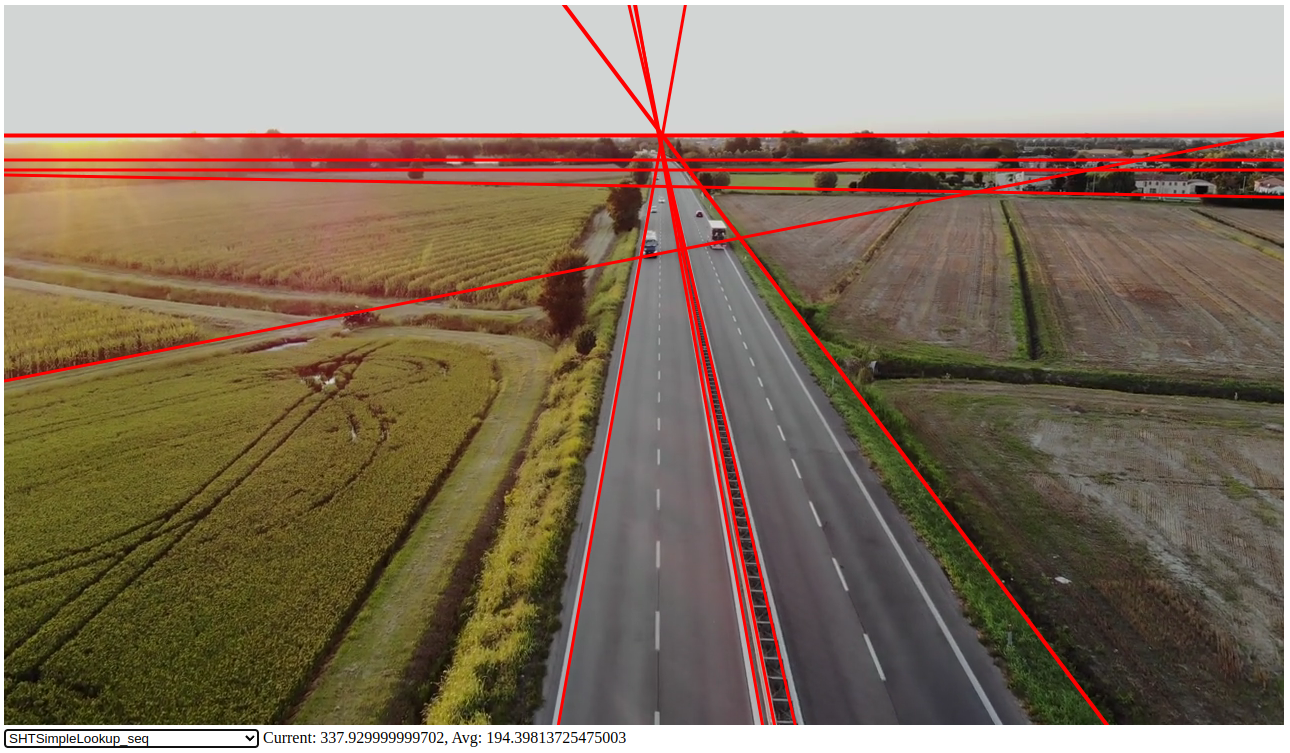
\includegraphics[width=\linewidth]{img/road.png}
        \caption{SHT}\label{fig:road}
    \end{subfigure}\hfill
    \begin{subfigure}{0.48\textwidth}
        \centering
        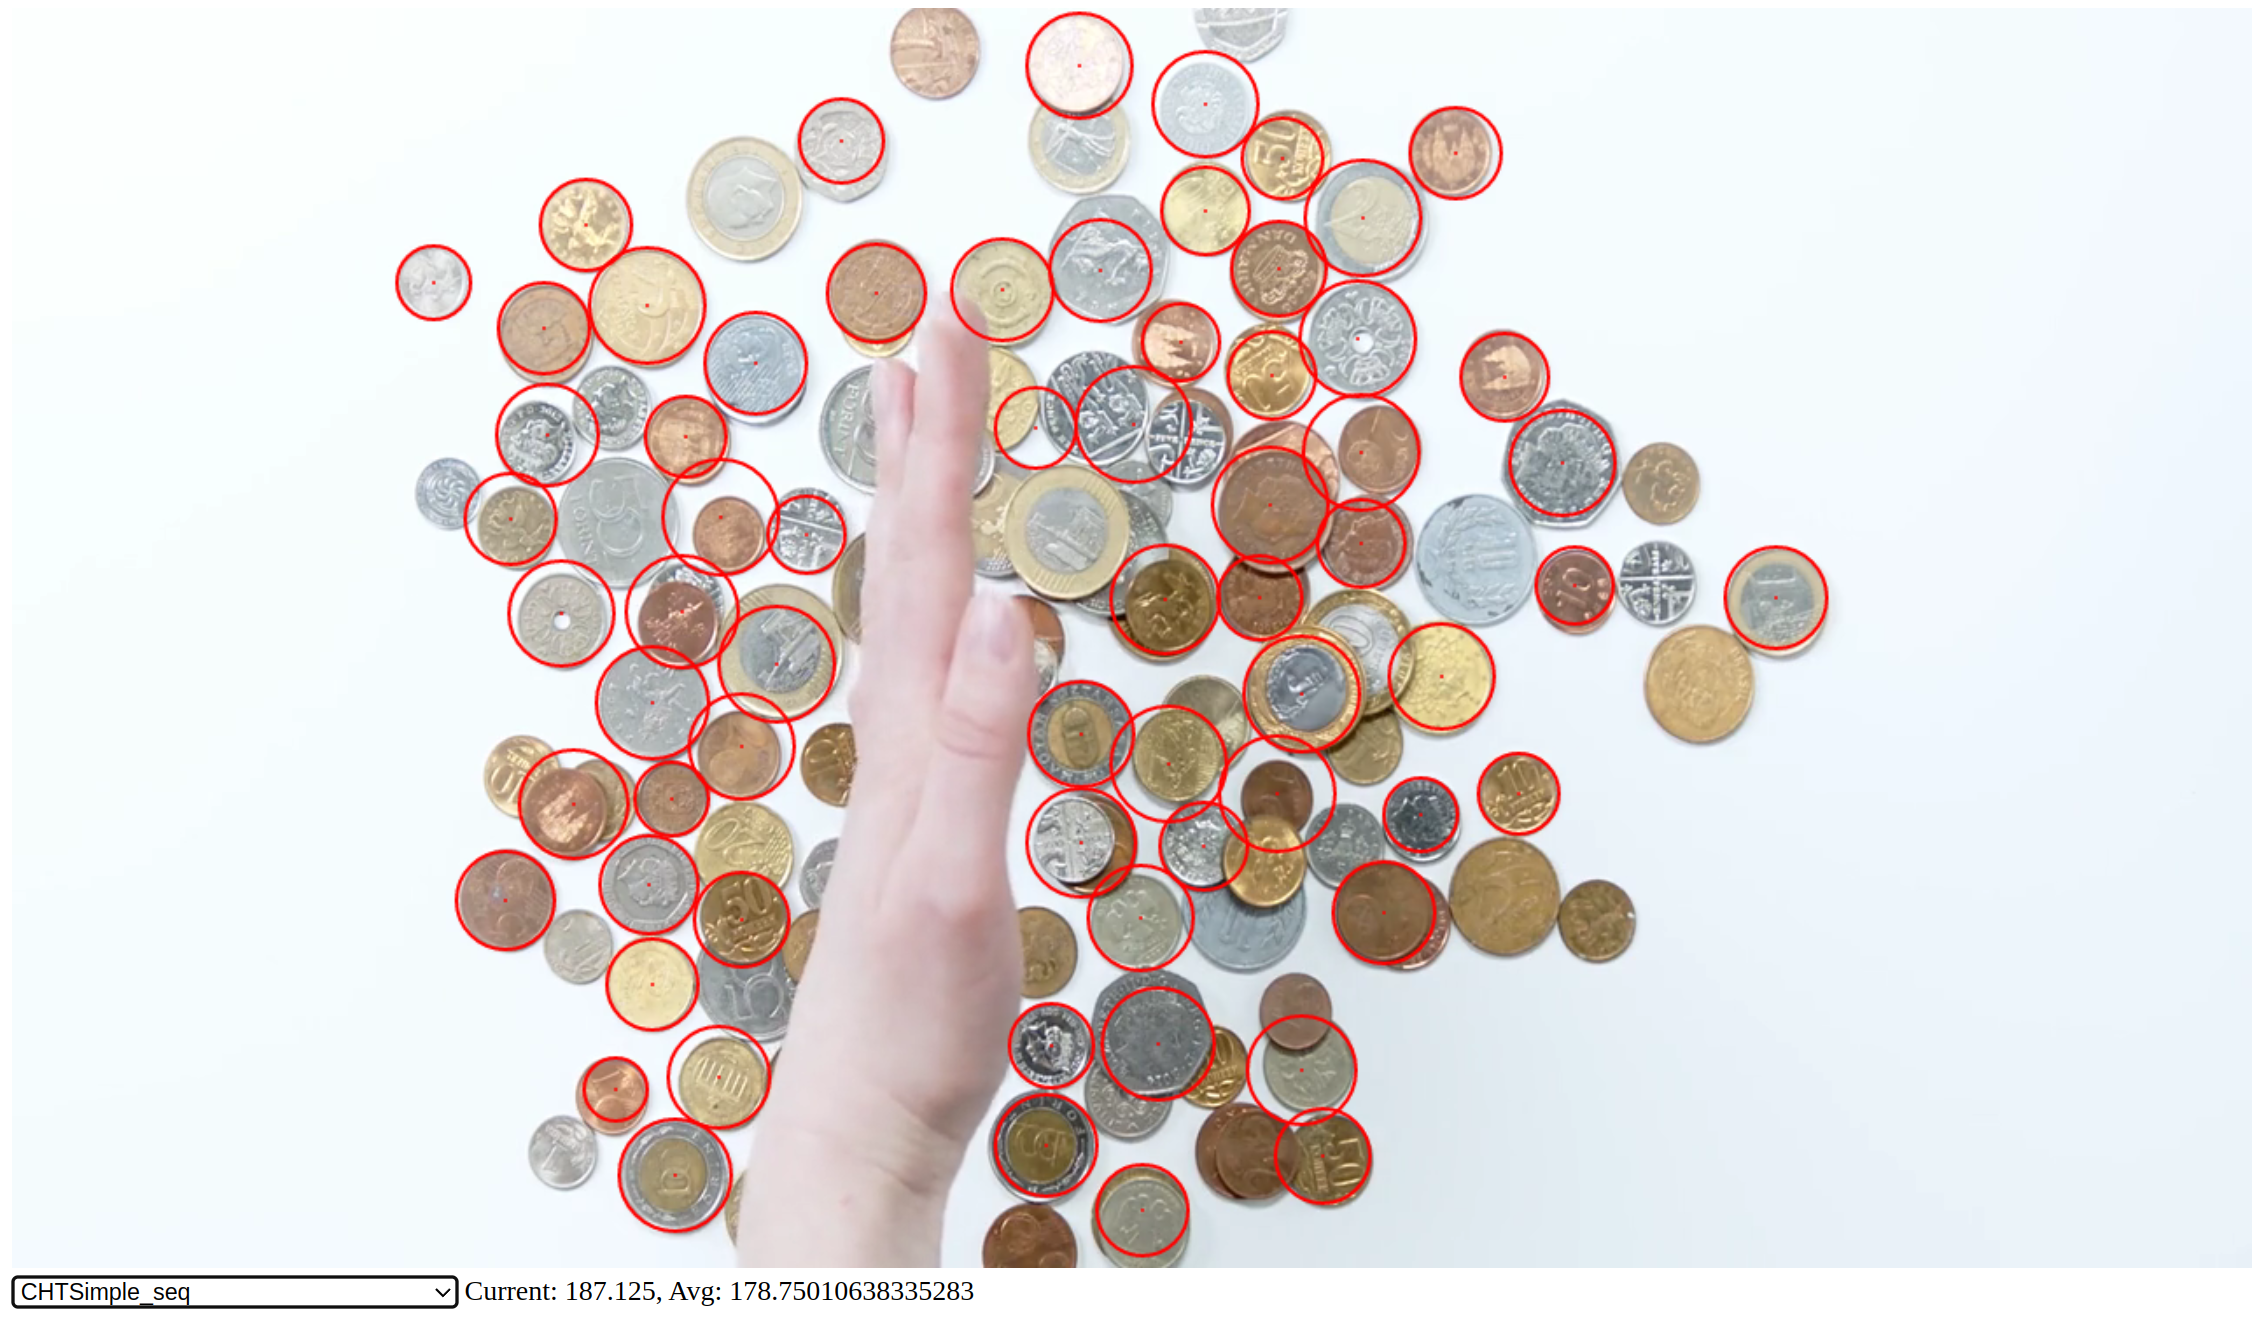
\includegraphics[width=\linewidth]{img/money.png}
        \caption{CHT}\label{fig:money}
    \end{subfigure}
    \caption{Wizualizacja wykrytych kształtów na podstawie obrazu z~kamery w~przeglądarce internetowej.}
    \label{fig:road-money}
\end{figure}

\begin{lstlisting}[language=JavaScript, float=ht, label=lst:loop, caption=Funkcja przetwarzająca w~pętli kolejne klatki obrazu z~kamery.]
async function loop() {
    if (resultCtx && imageCapture.value) {
        const imageBitmap = await imageCapture.value.grabFrame();
        resultCtx.drawImage(imageBitmap, 0, 0);
        image.data.set(resultCtx.getImageData(0, 0, width, height).data);
        const grayImage = image.grey();
        const canny = cannyEdgeDetector(grayImage, {
            lowThreshold: 50,
            highThreshold: 50,
        }) as Image;
        const inputImage = canny.data.map((v) => (v > 0 ? 1 : 0))
        await runHT(inputImage);
    }
    !stopLoop ? requestAnimationFrame(loop) : console.log("Loop stop");
}
\end{lstlisting}

Na listingu \ref{lst:loop} przedstawiona została główna pętla przetwarzania obrazu. Na podstawie tego przykładu i~wyników profilowania wykonania widać zatem, jak ważne jest zapewnienie wydajności całego łańcucha przetwarzania. Na rysunku \ref{fig:road-profiler} widać, że z~czasu przetwarzania, które trwało 173ms, przeglądarka poświęciła 120ms, czyli zdecydowaną większość, na wykonanie zewnętrznej i~niezoptymalizowanej pod względem wydajności metodzie \lstinline{CannyEdgeDetector} (69\% czasu). Wstępne przetwarzanie obrazu trwało 7.5ms (4\% czasu), a~implementowana detekcja linii 40ms (23\% czasu).

\begin{figure}[h]
    \centering
    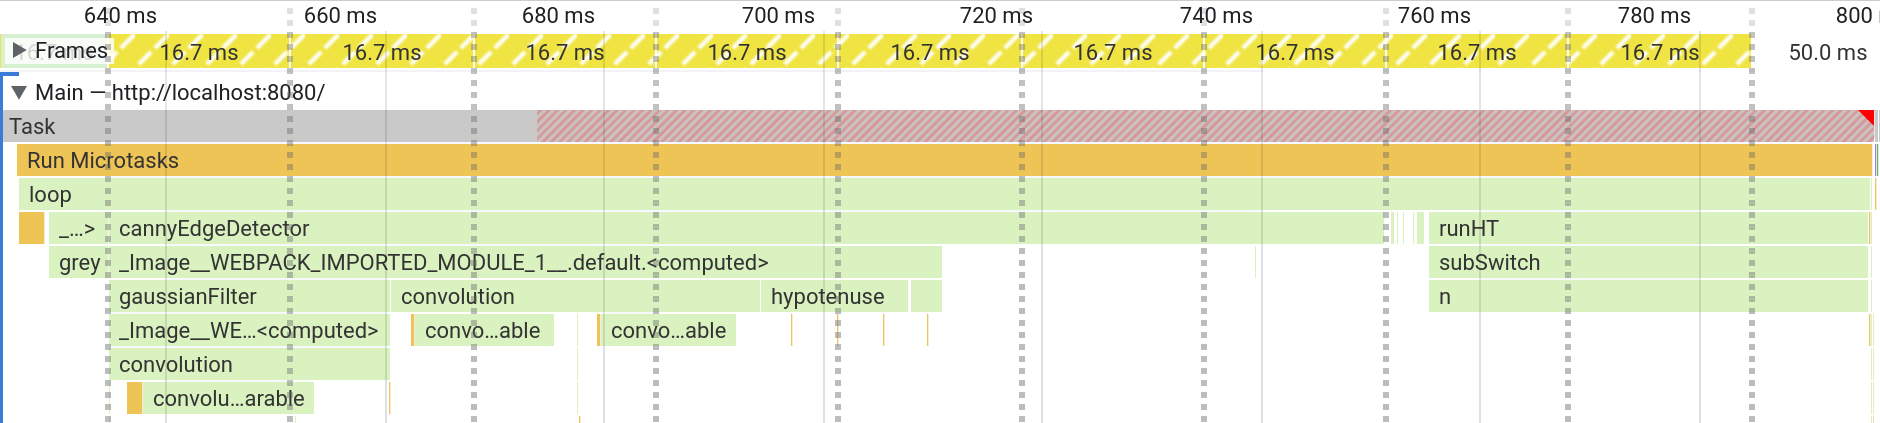
\includegraphics[width=\linewidth]{img/road-profiler.png}
    \caption{Wynik profilowania wykonania sekwencyjnego algorytmu SHT \textit{LUT} wraz z~procesem pozyskania obrazu, przetwarzania wstępnego, wykrywania krawędzi i~wyświetlenia wyników.}
    \label{fig:road-profiler}
\end{figure}

Ta próba implementacji procesu od pozyskania obrazu, przez jego przetwarzanie, aż do wyświetlenie wyników pokazuje nieprzystosowanie środowiska przeglądarki internetowej do przetwarzania obrazów. Również wiele do życzenia pozostawia cały ekosystem bibliotek, którym często brakuje kompatybilności i~popularności na tle ich odpowiedników w~języku Python. 
